\documentclass[../notes.tex]{subfiles}

\begin{document}
	
\section{Temperature and Energy Transfer}
Temperature is the average internal kinetic energy of an object.
The SI Unit of temperature in Kelvins ($K$).
However, Celsius is sometimes used.
\begin{equation}
	K = C + 273
\end{equation}

In general, temperature will aways attempt to reach thermal equilibrium.
Meaning that objects will aways try to reach the same temperature over time.

A temperature of $0 K$ is called absolute temperature. 
This is when the internal energy of a mas is zero.

\subsection{Internal Energy}
Substances consist of particles in constant random motion.
The internal energy of a molecule is the total potential and random kinetic energy of all the particles in a substance.

\subsection{Specific Heat Capacity}
The Specific Heat Capacity is defined as the amount of energy needed to raise a unit mass of an object by one Kelvin.
This equation models the relationship between change in temperature and energy.
\begin{equation}
	Q = mc\Delta T
\end{equation}
Where $Q$ is the energy required, $m$ is the mass, $c$ is the specific heat capacity, and $\Delta T$ is the change in temperature.

\subsection{Specific Latent Heat}
Latent heat is the amount of energy required to shift an object from one state to another.
This equation models the relationship between latent heat and energy.
\begin{equation}
	Q = mL
\end{equation}
Where $Q$ is the energy required, $m$ is the mass, and $L$ is the latent heat.

Latent heat of fusion is the energy require to change the phase from liquid to solid of 1kg of substance.
Latent heat of vaporization is the energy required to change the phase of 1kg of liquid into a gas.

\subsection{Phase Change Diagram}
This diagram shows the internal energy of a substance as it changes state.
\begin{figure}[h]
\begin{center}
	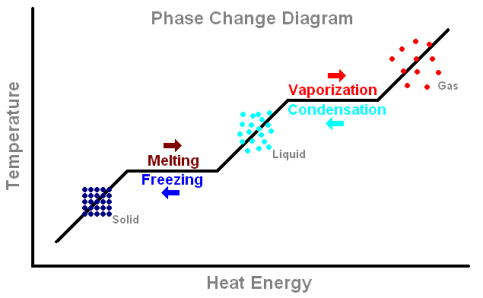
\includegraphics[width=\textwidth]{./figures/phase change diagram.png}
	\caption{A Phase Change Diagram}
\end{center}
\end{figure}

\section{Modeling a gas}

\subsection{Mole and the Avogadro Constant}
The mole is used for measuring the amount of substance.
A mol of gas contains $6.02 \cdot 10^23$ atoms.
This is also the Avogadro constant.

\subsection{Molar Mass}
The molar mass of an substance is the mass of one mol of said substance.
\begin{equation}
	\textrm{Mass of substance} = \textrm{Substance Molar Mass} \times \textrm{Mols of Substance}
\end{equation}

\subsection{Ideal Gas Law}
The Ideal Gas Law sum up the relationship between pressure, volume, temperature, and moles of molecules of a gas.
\begin{equation}
	pV = nRT
\end{equation}
Where $p$ is pressure (SI Unit is Pascals or $Pa$), $V$ is volume, $n$ moles of molecule (SI Unit in moles or Mol), $R$ is the ideal gas constant ($8.3145 \cdot 10^3$), and $T$ is the temperature (in Kelvins).

\subsection{Assumptions of an Ideal Gas}
\begin{itemize}
	\item A gas consist of many tiny molecules in random motion
	\item Each molecule has negligible volume when compared with the volume of the gas
	\item Molecules undergo perfectly elastic collisions
	\item There is no intermolecular force, the energy of the molecules is only kinetic
	\item The duration of a collision is negligible compared with the time between the collisions
	\item Forces of individual molecules with average out to an uniformed pressure
\end{itemize}

\subsection{Total Internal Energy of an Ideal Gas}
The total internal energy of an ideal gas is the sum of the average random kinetic energy of each particle inside the gas.
\begin{equation}
	\sum KE = \frac{3}{2} N k_B T
\end{equation}
Where $k_B$ is the Boltzmann Constant, $N$ is the amount of particles, and $T$ is the temperature.

Note, the internal energy of each individual particle is the equation above without $N$.
\begin{equation}
	KE = \frac{3}{2} k_B T
\end{equation}

\subsection{Real Gases}
Ideal gas is ideas.
Ideal gases cannot be liquefied.
Thus, as a gas near high pressure or low temperatures, it may behave like a real gas instead of an ideal gas.
A real gas is a non idea gas.

\end{document}
